%% template by Michael Shell
%% See: 
%% http://www.michaelshell.org/
%% for current contact information.
%%
%% This is a skeleton file demonstrating the advanced use of IEEEtran.cls
%% (requires IEEEtran.cls version 1.8b or later) with an IEEE Computer
%% Society journal paper.
%%
%% Support sites:
%% http://www.michaelshell.org/tex/ieeetran/
%% http://www.ctan.org/pkg/ieeetran
%% and
%% http://www.ieee.org/

%%*************************************************************************
%% Legal Notice:
%% This code is offered as-is without any warranty either expressed or
%% implied; without even the implied warranty of MERCHANTABILITY or
%% FITNESS FOR A PARTICULAR PURPOSE! 
%% User assumes all risk.
%% In no event shall the IEEE or any contributor to this code be liable for
%% any damages or losses, including, but not limited to, incidental,
%% consequential, or any other damages, resulting from the use or misuse
%% of any information contained here.
%%
%% All comments are the opinions of their respective authors and are not
%% necessarily endorsed by the IEEE.
%%
%% This work is distributed under the LaTeX Project Public License (LPPL)
%% ( http://www.latex-project.org/ ) version 1.3, and may be freely used,
%% distributed and modified. A copy of the LPPL, version 1.3, is included
%% in the base LaTeX documentation of all distributions of LaTeX released
%% 2003/12/01 or later.
%% Retain all contribution notices and credits.
%% ** Modified files should be clearly indicated as such, including  **
%% ** renaming them and changing author support contact information. **
%%*************************************************************************

\documentclass[journal]{IEEEtran}
\usepackage{booktabs} % required for tables
\usepackage[T1]{fontenc} % Output font encoding for international characters
\usepackage{siunitx}
\usepackage{amsmath}
\usepackage{graphicx}
\usepackage{caption}
\usepackage{hyperref}

%
\ifCLASSOPTIONcompsoc
  % The IEEE Computer Society needs nocompress option
  % requires cite.sty v4.0 or later (November 2003)
  \usepackage[nocompress]{cite}
\else
  % normal IEEE
  \usepackage{cite}
\fi
% \usepackage[backend=bibtex,style=authoryear,natbib=true]{biblatex} % Use the bibtex backend with the authoryear citation style (which resembles APA)

% \addbibresource{main.bib} % The filename of the bibliography

\newcommand\MYhyperrefoptions{bookmarks=true,bookmarksnumbered=true,
pdfpagemode={UseOutlines},plainpages=false,pdfpagelabels=true,
colorlinks=true,linkcolor={black},citecolor={black},urlcolor={black},
pdftitle={TDoA_project_report},
pdfsubject={TDoA trajectory reconstruction},
pdfauthor={Morhunenko Mykola},
pdfkeywords={TDoA}}

% correct bad hyphenation here
\hyphenation{}

\begin{document}

\title{TDoA trajectory reconstruction}
\author{Morhunenko Mykola}
% make the title area
\maketitle

% =================================================================================
\IEEEraisesectionheading{\section{Introduction}\label{sec:introduction}}
Within the subject "Diagnostics and testing", there is a compulsory semester project for each student on a chosen topic.
The project "Time-Difference-of-Arrival (TDoA) trajectory reconstruction" sounded the most algorithmic among others, so it was chosen. 
The main goal is to find a trajectory of a moving object (i.e. tag) repeatedly transmitting a signal, using a set of given fixed-position receivers (i.e. anchors).

% =================================================================================
\section{Problem description}
\label{sec:problem}

\begin{figure}[ht]
    \centering
    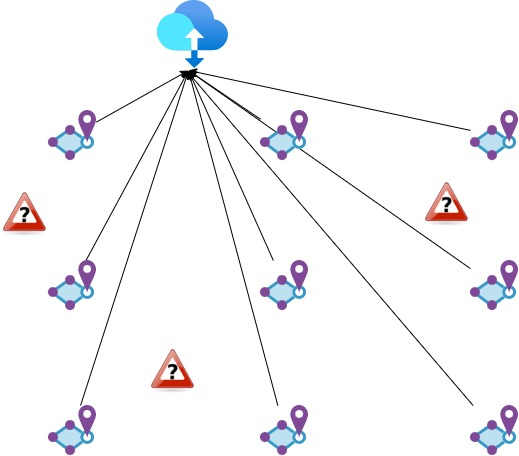
\includegraphics[width=0.30\textwidth]{graphics/scheme.jpg}
    \caption{The model of the experiment. Nine anchors connected in a network to some main recording computer, and some number of unknown moving objects (in both files, there are two of them, number 5 and number 30).}
    \label{fig:3D_map}
\end{figure}

Indoor localisation is a popular and widely researched topic nowadays.
TDoA localisation is based on periodically sending a message by a tag to a set of fixed anchors. 
The theory behind it is elementary and relies on a few facts: the speed of a signal is the speed of light (so it's known), and the time of sending and receiving the message both are known.
Then the task is just a school geometry problem - having a few equations find the unknown variable.

But in the real world, everything is not as perfect and smooth as in theory, so while implementing this method, some more problems should be solved.
The first one - travelling at the speed of light is a sensitive process that can not be measured as precisely, so exact real-time ultra wide band (UWB) transmitters with precise clocks are needed. 
It was solved by people who were setting up the experiment and have chosen DW1000 chips.
The second problem - these clocks should be somehow synchronised because there is no perfect physical mechanism, and without the synchronisation, they are useless.
The third one - due to possible reflections from different surfaces, data transfer errors, oscillations, etc., the recorded time of travelling from the tag to anchors can be changed or have some noise.

% =================================================================================
\section{Set tasks}
\label{sec:set_tasks}
The task was divided into smaller steps to make it easier to solve the main task.
\begin{itemize}
    \item Given datasets analyses;
    \item Research into related works;
    \item Time synchronisation problem;
    \item Known object localisation;
    \item Unknown object localisation;
\end{itemize}

% =================================================================================
\section{Data description}
\label{sec:data_desc}
\begin{figure}[ht]
    \centering
    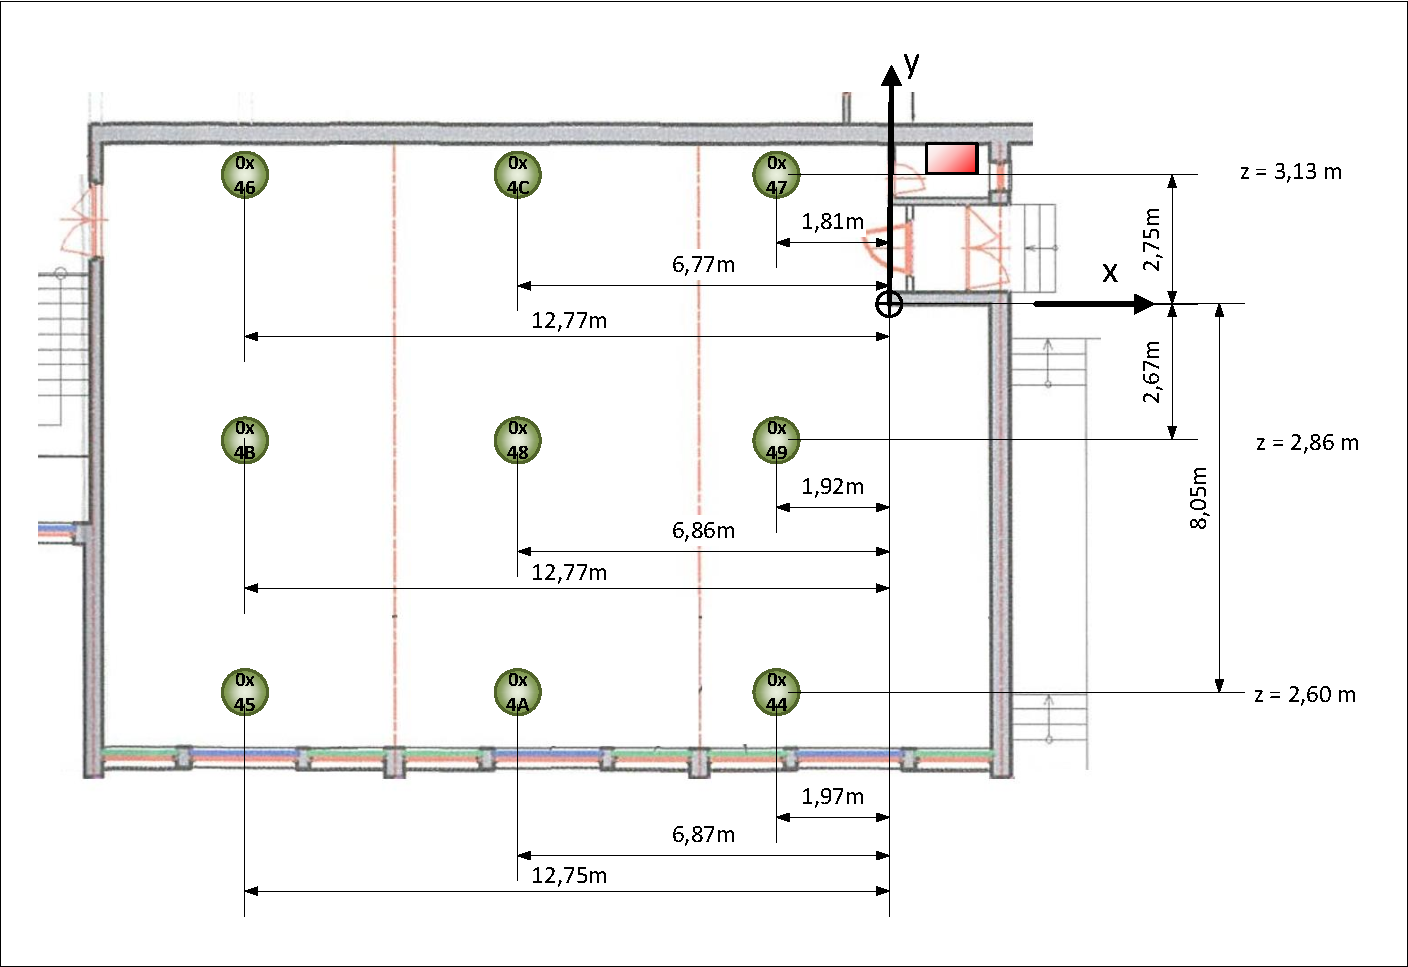
\includegraphics[width=0.48\textwidth]{graphics/UWB_map.pdf}
    \caption{The indoor map of the anchors is shown in the image. Nine anchors with hexadecimal identifiers are located in a 3x3 grid, each row at a different height.}
    \label{fig:UWB_map}
\end{figure}
\begin{figure}[ht]
    \centering
    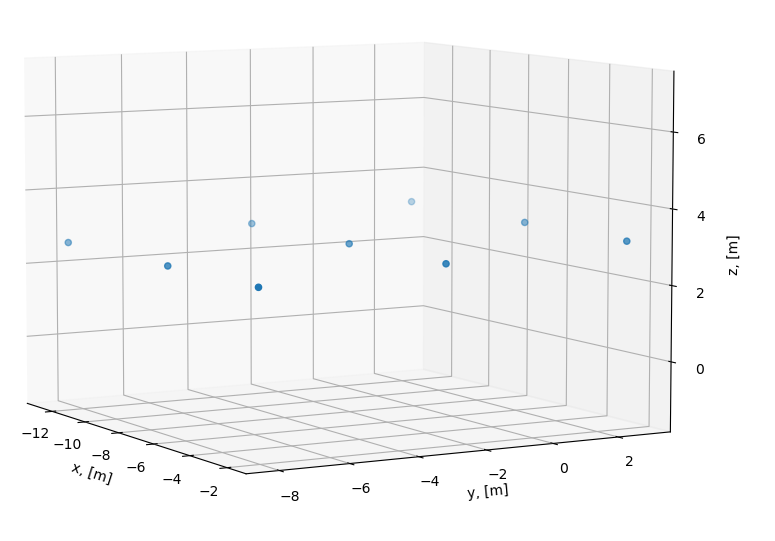
\includegraphics[width=0.30\textwidth]{graphics/room3D.png}
    \caption{The indoor map of the anchors in 3D.}
    \label{fig:3D_map}
\end{figure}

Along with the project assignment, two files from the real-world experiments, and an indoor map (see \autoref{fig:UWB_map}) were provided. So the room in 3D can be visualized as in \autoref{fig:3D_map}, where all anchors are arranged in three rows, each on a different height.

For each experiment, there are "blinks" and "syncs" files.
"syncs.csv" files contain synchronisation messages between anchors in the form "addr\_tx, addr\_rx, ts\_tx, ts\_rx, the timestamp",  where the first two columns are addresses of the transmitter and receiver, respectively, next two columns correspond to the timestamps of the recording module DWM1000 on each anchor, which measures time in its own units (here and further - $[\SI{}{dw}]$) where $\SI{1}{dw} = \frac{1}{(128*499,2*10^6)}\SI{}{s}$. 
The last column corresponds to the timestamp of an experiment recording system, which runs on Unix, time in $[\SI{}{ms}]$.
"blinks.csv" files contain location messages between an unknown moving object and anchors in the format "addr\_tx, addr\_rx, ts\_rx, ts\_tx, id" where the first two columns are addresses of transmitter and receiver, respectively, next two columns are corresponding timestamps of message transmission and receiving, and the last column corresponds to the message id.

\begin{figure}[ht]
    \centering
    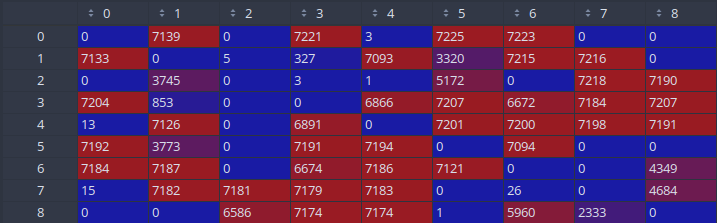
\includegraphics[width=0.48\textwidth]{graphics/stat_exchange.png}
    \caption{The number of messages in a whole file sent from the node $i+68$ to the node $j+68$. Node 0 corresponds to 68, node 8 - to 76.}
    \label{fig:tbl}
\end{figure}
\begin{figure}[ht]
    \centering
    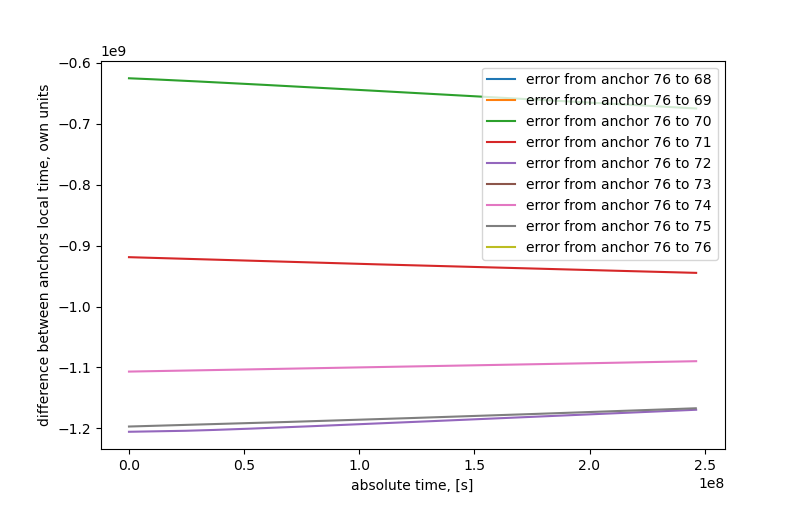
\includegraphics[width=0.48\textwidth]{graphics/errors.png}
    \caption{The error between the time frames of anchor 76 and each other anchor in the whole dataset.}
    \label{fig:stat_all}
\end{figure}
\begin{figure}[ht]
    \centering
    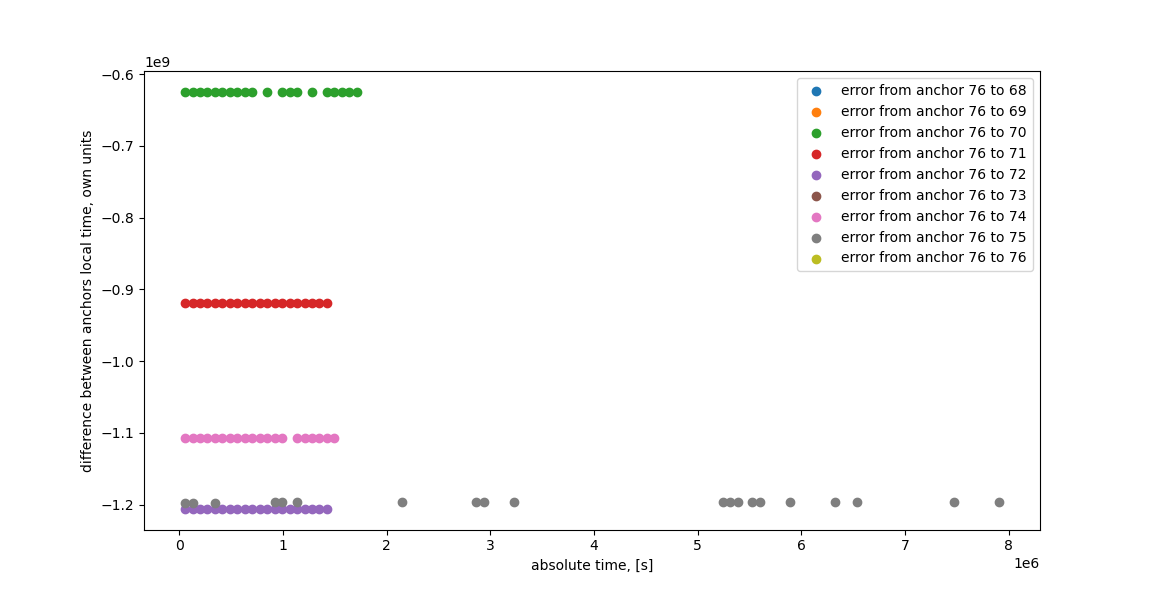
\includegraphics[width=0.48\textwidth]{graphics/errors_scaled.png}
    \caption{The error between the time frames of anchor 76 and each other anchor (y axis) with respect to the timestamp of 76th anchor (x axis), first 100 in the dataset.}
    \label{fig:stat_cropped}
\end{figure}
% \begin{figure}[ht]
%     \centering
%     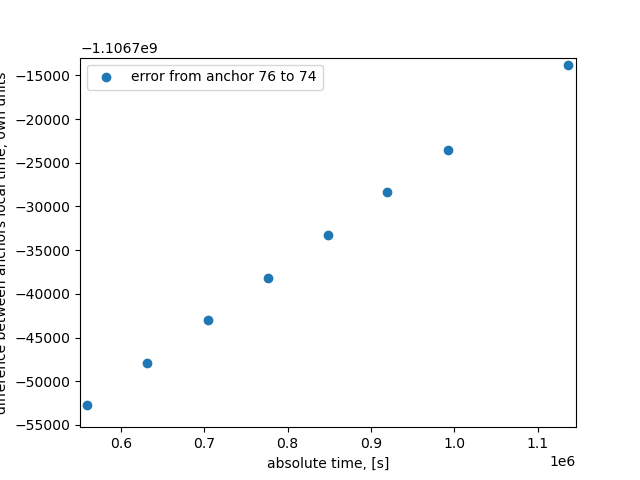
\includegraphics[width=0.48\textwidth]{graphics/errors_close.png}
%     \caption{The error between the time frames of anchor 76 and 74 (y axis) with respect to the timestamp of 76th anchor (x axis).}
%     \label{fig:stat_cropped_alot}
% \end{figure}

The number of messages coming from each to each node is shown in the \autoref{fig:tbl}. From this table its obvious that not all anchors exchange messages - for example the anchor $70$ is almost isolated (only two connections), but such anchors as $69, 71, 72 ,73, 74$ are well-connected (only three missing connections).

The time difference (error) between 75 and each other anchor is shown in the \autoref{fig:stat_all}. Its shown that the error is not constant or linear. The first 100 computed errors are shown in \autoref{fig:stat_cropped}. The conclusion is that sync messages are not actually periodic and there is a lot of data loss in the process of communication between anchors.

% =================================================================================
\section{Related works}
\label{sec:ps}
The TDoA indoor localisation is a well-described topic, but in most cases, it's done in 2D due to different singularities and issues in 3D. In \cite{Laaraiedh2009}, it is written how to overcome them. 

The general idea and method of TDoA self-localisation are well-described in a \cite{Keefe2017}. 
In \cite{Yuzan2019}, there is a proposed online time-synchronization and location estimation method. 
Still, it can not be implemented for the post-processing because it needs some external experiment setup for all anchors.

The implemented localisation algorithms are taken from \cite{Weng2011}, and \cite{Yuzan2019}.

% =================================================================================
\section{Method}
\label{sec:method}

\subsection{Trajectory reconstruction using nonlinear least-squares}
\label{sec:traj_recon}
Here and further consider already synchronised time with respect to the main anchor.
Let any two non-similar anchors be $i$ and $j$ located on a distance $d_{ij}$.
Timestamps of received signals from the tag by each anchor are denoted as $t_i$ and $t_j$.
The time difference between the arrival of the two signals is
\begin{equation}
    {t}_{ij} = t_i - t_j.
    \label{eq:dt1}
\end{equation}
From another side, let us consider the coordinates of a moving object as $(x, y, z)$, coordinates of two anchors as $(x_i, y_i, z_i)$ and $(x_j, y_j, z_j)$ respectively.
The distance from a tag to each anchor can be written as
\begin{equation}
    d_i = \sqrt{(x-x_i)^2 + (y-y_i)^2 + (z - z_i)^2}.
    \label{eq:dist}
\end{equation}
Considering the time-velocity relation (distance = velocity * time) 
\begin{equation}
    \label{eq:ddcdt}
    {d}_{ij} = d_i - d_j = c{t}_{ij},
\end{equation}
and the equation \eqref{eq:dt1}, let us define the function f:
\begin{equation}
    \label{eq:f}
    f = d_j - d_i - c (t_j - t_i) = 0.
\end{equation}
Where both $t_j$ and $t_i$ are given, $c$ is a speed of a signal (speed of light), and $d_i, d_j$ together contain three unknowns. 

To find them, at least three such equations are needed, which corresponds to at least three anchors.
This problem is already formulated as a non-linear least squares (NLLS) problem so that it can be solved with any optimizer for such a task.

The gradient of $f$ needed for NLLS can be computed as:
\begin{equation}
    \nabla f(\left.x, y, z\right)=\left[\begin{array}{c}
    \dfrac{\partial f}{\partial x}\\
    \dfrac{\partial f}{\partial y}\\
    \dfrac{\partial f}{\partial z}
\end{array}\right] = \left[\begin{array}{c}
    \frac{x-x_j}{d_j} - \frac{x-x_i}{d_i}\\
    \frac{y-y_j}{d_j} - \frac{y-y_i}{d_i}\\
    \frac{z-z_j}{d_j} - \frac{z-z_i}{d_i}
    \end{array}\right].
\end{equation}

\subsection{Linear Closed-Form Solution}
Another implemented method is much easier in algebra but needs at least four anchors to work.
Assume the anchor with index $0$ as the main anchor with coordinates $(x_0, y_0, z_0))$.
Having one main anchor and $N-1$ other anchors with indexes $i=1 \ldots N$, there will be $N-1$ equations of a form \autoref{eq:ddcdt} for distances from the main to $i-th$ anchor:
\begin{equation}
    \begin{array}{cc}
        (x-x_0)^2 + (y-y_0)^2 + (z-z_0)^2 - d_0^2 = 0\\
        \vdots \\
        (x-x_N)^2 + (y-y_N)^2 + (z-z_N)^2 - (d_1 + d_{1N}) = 0 
    \end{array}
\end{equation}
After subtracting the first equation from all others, the result will be the set of equations that, after simplification, can be rewritten as a set of linear equation
\begin{equation}
    A\vec{x} = b,
\end{equation}
where
\begin{equation}
    A = \left[ \begin{array}{cccc}
         x_0 - x_1 & y_0 - y_1 & z_0 - z_1 & d_01  \\
         \vdots & \vdots & \vdots & \vdots \\
         x_0 - x_N & y_0 - y_N & z_0 - z_N & d_0N  \\
    \end{array} \right],
\end{equation}
\begin{equation}
    \vec{x} = \left[ \begin{array}{c}
         x \\ y \\ z \\ d_0
    \end{array} \right],
\end{equation}
\begin{equation}
    b = \left[ \begin{array}{c}
         b_1 \\ b_2 \\ \vdots \\ b_N
    \end{array} \right],
\end{equation}
and 
\begin{equation}
    b_i = \frac{1}{2} \left( \begin{array}{c}
         x_0^2 - x_i^2 + y_0^2 - y_i^2 + z_0^2 - z_i^2 + d_{0i}^2
    \end{array} \right).
\end{equation}

So that can be solved using the linear least-squares method:
\begin{equation}
    x = (A^{T}A)^{-1}A^{T}b.
\end{equation}

\subsection{Time synchronisation}
\label{sec:time_sync}

Time synchronisation is essential for this task because without it, results have no sense.
Firstly, the memoisation was chosen for the time synchronization because its easy to implement and check how it works.
Let $T_{ij}$ be the time of flight from anchor $i$ to $j$, the main anchor index to be $m$.
If clocks on two anchors are perfectly synchronized, the ideal timestamps of sending a message from $t_m$ to $t_i$ would be:
\begin{equation}
    \label{eq:sync_ideal}
    t_{i}^* = t_m + T_{mi},
\end{equation}
but in the real world, this time would be
\begin{equation}
    \label{eq:sync}
    t_{i}^{'} = t_m + T_{mi} + e_{mi},
\end{equation}
where $e_{mi}$ stands for some error.

The array $A_{cor}$ contains time corrections for each anchor with respect to the main anchor. 
Continuing analysing equations \eqref{eq:sync_ideal} and \eqref{eq:sync}, the time correction in case the message was sent from the main anchor can be found as
\begin{equation}
    t_{c} = t_i^{'} - t_i^{*} = A_{cor}[i]
\end{equation}
and the matrix $A_{cor}$ can be updated.

The same is true if the sync message was transferred from any $t_i$ to $t_m$; the time correction can be found as
\begin{equation}
    t_i^{*} = t_m - T_{im},
\end{equation}
\begin{equation}
    t_i^{'} = t_m - T_{im} + e_{im},
\end{equation}
\begin{equation}
    A_{corr}[i] = t_i^{'} - t_i^{*},
\end{equation}
then at any time $t \approx t_i$ can be transformed to the main anchors' time domain $t^m$ as
\begin{equation}
    t_i^{m} = t_i + A_{corr}[i].
\end{equation}

Not all anchors receive every synchronisation signal, so the matrix $A_{cor}$ updating can be accelerated by considering pairwise messages between any two anchors $i$ and $j$, the sync message going from $i \rightarrow j$. If the anchor $i$ is not yet synchronised with the network, we can update only it. In the main anchor time domain, it is as follows:
\begin{equation}
    t_i^{*} = t_j + A_{cor}[j] - T_{ij},
\end{equation}
\begin{equation}
    t_i^{'} = t_j + A_{cor}[j] - T_{ij} + err_{ij},
\end{equation}
\begin{equation}
    A_{cor}[i] = t_i^{'} - t_i^{*}.
\end{equation}

In the opposite situation, when the anchor $j$ is not yet synchronised,
\begin{equation}
    t_j^{*} = t_i + A_{cor}[i] + T_{ij},
\end{equation}
\begin{equation}
    t_j^{'} = t_i + A_{cor}[i] + T_{ij} + err_{ij},
\end{equation}
\begin{equation}
    A_{cor}[j] = t_j^{'} - t_j^{*}.
\end{equation}

\subsection{Error prediction}
\begin{figure}[ht]
    \centering
    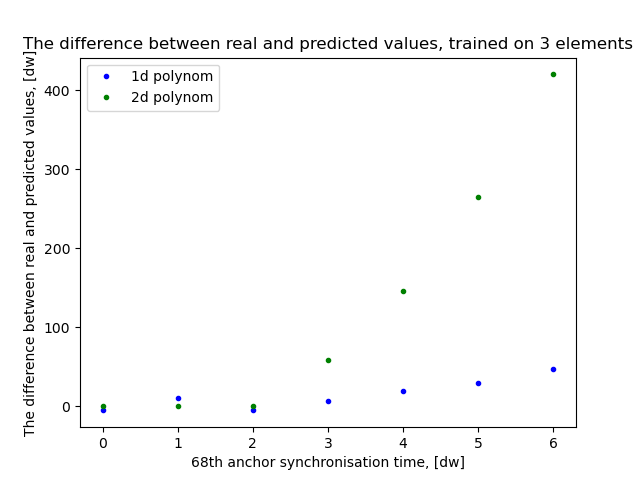
\includegraphics[width=0.48\textwidth]{graphics/68_prediction.png}
    \caption{The difference between the real and predicted values. First three values are training values.}
    \label{fig:pred}
\end{figure}
To improve the time synchronisation, the simple polynom fit and prediction is used. 
In \autoref{fig:pred} it is shown that 1d line is good enough estimate for the function on a short distance.
Given even two points, the line going through them can be estimated and than the future point can be predicted.
Given three points the data will not be overfeated and the prediction result can be improved, it will ignore some minor oscillations and noise.
So it was decided to use a linear prediction to find the time difference between any two anchors by saving the last 3 error corrections between them.
If the history is not complete (there were less then 3 messages processed) the data from $A_{cor}$ table can be used.
% =================================================================================
\section{Implementation}
% \label{sec:impl}
% \begin{figure}[ht]
%     \centering
%     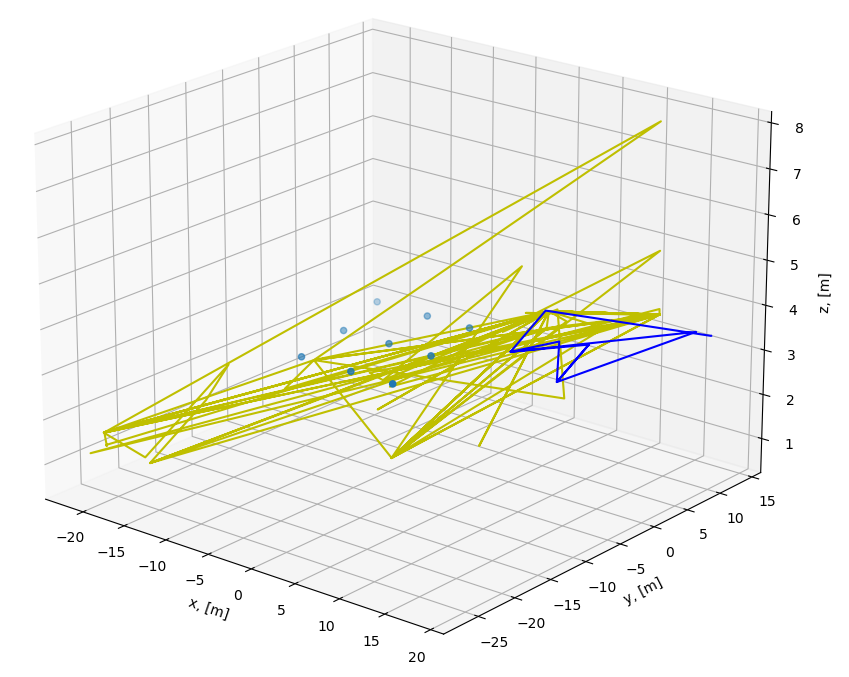
\includegraphics[width=0.48\textwidth]{graphics/walls5_res.png}
%     \caption{The result of the trajectory reconstruction from the walls5 dataset.}
%     \label{fig:walls_5}
% \end{figure}
% \begin{figure}[ht]
%     \centering
%     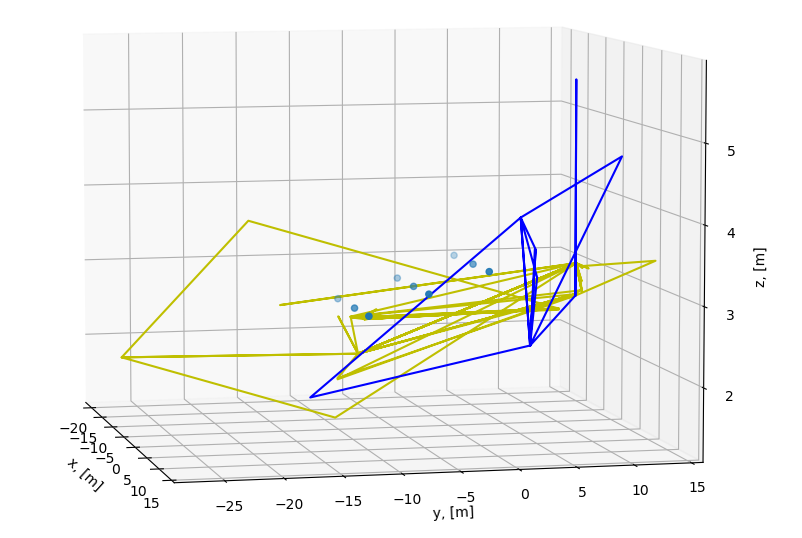
\includegraphics[width=0.48\textwidth]{graphics/cold_start.png}
%     \caption{The result of the trajectory reconstruction from the cold\_start dataset.}
%     \label{fig:cold_start}
% \end{figure}


Everything was implemented in Python using 'numpy' and 'scipy' libraries.
The first phase is data preprocessing. 
In each file repeating rows are eliminated (because they are useless), and each file is sorted with respect to the timestamp.
After that, there is an iteration through the whole syncs file to keep track of the time synchronisation, and when there are blinks - they are processed concerning the current inner state of the system.
If the signal was sent by the tag at different timestamps or less than three anchors had received the message, it is ignored, and the corresponding message is displayed.

The class 'AnchorsField' is the main class that keeps track of the matrix $A_{corr}$ as an inner parameter of the field.
At each point of time, the location of the tag from a given data can be found as a result of solving the NLLS with the optimiser \href{https://docs.scipy.org/doc/scipy/reference/generated/scipy.optimize.least_squares.html#scipy.optimize.least_squares}{'scipy.optimize.least\_squares'}.

% The obtained result from the 'walls5' dataset is shown in the \autoref{fig:walls_5}, and the obtained result from the 'cold\_start' dataset is shown in the \autoref{fig:cold_start}.


The whole implementation is available by this link ":TODO link"
% =================================================================================
\section{Error measurement}
\label{sec:error}

% =================================================================================
\section{Conclusion}
The conclusion goes here.

% =================================================================================
\bibliography{main}{}
\bibliographystyle{ieeetr}
\cleardoublepage

\end{document}

